

\section{Contact Dynamics}


Up to now we have introduced two different types of approaches to molecular dynamics simulations: finite time steps integration and event driven algorithms. The first explicitely solves the equations of motion, while the second makes  use of some collision rules to predict the trajectories. Finite time steps integration methods are good for soft potentials or precise predictions of relatively small systems (e.g. the solar system), while event driven is suited for rigid bodies and large systems of particles with simple interaction (e.g., elastic and quasi instantaneous scattering). The drawbacks of event driven dynamics are that it is very inefficient for high densities (the particles keep colliding all the time) and it is completely useless for the simplest of all cases: contact of particles at rest. This is a very important issue since there are many cases in which one wants to simulate precise interactions of objects and particles that are constantly (or partially) in contact. An example for this are robotic actuators that are composed by few parts but have to reach high precision in spatial displacement or application of forces. Think about the employment of robotic actuators in surgery. None of the methods we discussed until now is suited for this, and therefore \emph{contact dynamics}.



Petr L\"otstedt was one of the first to conceive the field but he never put many of his ideas into practice. The one that really made the method famous, Jean Jacques Moreau, was a professor in numerical analysis specialized in elliptic equations. He taught in Montpellier, and after his retirement he started developing the programs on his own and worked almost until his death in the early 2014, at the age of 90  \citep{moreau_comm}. 


\vspace{.5cm}
The origin of contact dynamics lies in non-smooth mechanics. Originally formulated by Alberto Signorini, the \emph{ambiguous boundary condition problem} what is known today as the \emph{Signorini Problem} is a classic problem.  


\vspace{0.2cm}
\noindent
\begin{minipage}{\textwidth}
\begin{minipage}{0.48\textwidth}
The question is what shape an elastic body assumes if it is constrained by some rigid bodies. Of course, the objects are not allowed to overlap (except in very special situations). An example is a rubber object laying on a table. This gives rise to the Signorini Graph: If there is no overlap or contact between the surfaces of the objects, there are no  forces between them either. On the contrary, if there are any forces between the objects, then the distance between the surfaces is zero. This causes a discontinuity in the force, hence a problem for any simulation (Fig. \ref{fig:signorini}).
\end{minipage}
\hfill
\begin{minipage}{.5\textwidth}
  \centering
  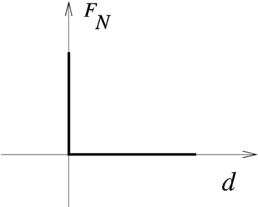
\includegraphics[width=.75\textwidth]{pics/signorini.jpeg}
  \captionof{figure}{Signorini Graph}
  \label{fig:signorini}
\end{minipage}
\end{minipage}
\vspace{0.1cm}


\noindent
\begin{minipage}{\textwidth}
\begin{minipage}{0.48\textwidth}
Related to this problem is the \emph{Coulomb-Graph}. An example of this is the friction between two objects that are in contact. If the relative velocity is zero, there is no force, if the velocity assumes any value which is not zero, then the friction suddendly changes. As one can see, the problem can be reformulated with forces or velocities but the concept is the same.
\end{minipage}
\hfill
\begin{minipage}{.5\textwidth}
  \centering
  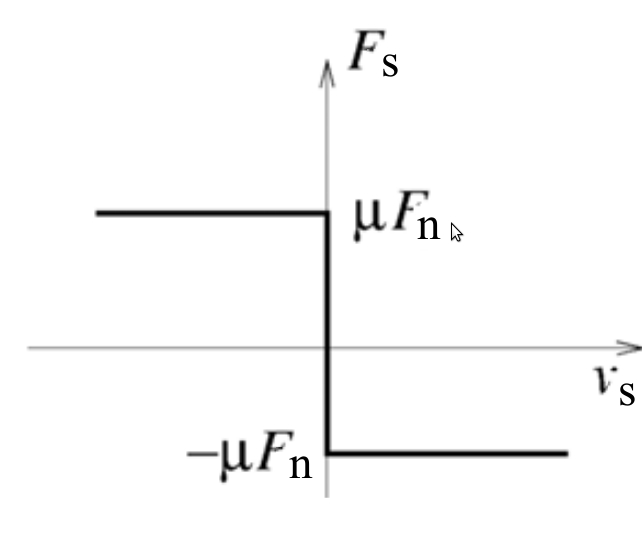
\includegraphics[width=.75\textwidth]{pics/signorini2.jpeg}
  \captionof{figure}{Coulomb Graph}
  \label{fig:signorini2}
\end{minipage}
\end{minipage}
\vspace{0.1cm}

\subsection{1D Contact}
As a start, we will first neglect friction between particles with relative velocity $v_s$ and only consider normal forces at contact. As we said in our assumptions, particles are not allowed to overlap. The costraint forces must therefore be imposed in such a way that they compensate all the forces that would make the particles overlap.  There are two issues of which one should be aware: first of all, the forces neither do act before the contact happens, nor they do once the distance after an overlap is restored. In fact there is never an overlap. The scheme must be therefore implicit, since we cannot calculate what forces are needed to restore the contact from an overlap. In our implicit Euler integration this would translate to:


\begin{align*}
\vec{v}_i \kl{t+\Delta t} &=  \vec{v}_i \kl{t} + \frac{1}{m_i} \underbrace{\vec{F}_i \kl{t+\Delta t}}_{\vec{F}_i^{\,\text{ext}} + \vec{R}_i^{\,\text{constr}}} \Delta t \\
\vspace{0.1cm}
\vec{r}_i \kl{t+\Delta t} &=  \vec{r}_i \kl{t} + \vec{v}_i \kl{t+\Delta t} \Delta t 
\end{align*}
The forces are a combination of the external and constraint forces.

The second issue is that the constraint forces do not act on the center of mass of the particle; they act locally at the contact point. Usually for rigid bodies one can calculate all the forces as acting at the center of mass. This is not the case anymore. We will therefore transform all the equations that we usually have for the center of mass to a new set of equations for the contact point and the contact variables.


As an example, we will examine the contact of two one-dimensional bodies. The matrix $H$ transforms the contact forces (that are local forces) into forces between the particles. The matrix $H^T$ does the same for the velocities:

\begin{equation*}
v_n^{\text{loc}} = v_2-V_1 = \ekl{-1,1} \cvec{v_1}{v_2} = H^T \cvec{v_1}{v_2}
\end{equation*}
\begin{equation}
\cvec{R_1}{R_2} = \cvec{-R_n^{\text{loc}}}{R_n^{\text{loc}}} =  \cvec{-1}{1} R_n^{\text{loc}} = HR_n^{\text{loc}}
\label{transf_h}
\end{equation}
These two coupled equations correspond to the usual Newton's equations. In vectorial form we have:



\begin{equation}
\frac{\text{d}}{\text{dt}}\cvec{R_1}{R_2} =\frac{1}{m} \kl{\cvec{-R_1}{R_2} +\cvec{F_1^{\text{ext}}}{F_2^{\text{ext}}}} 
\end{equation}
We now can insert the contact quantities using the transformation given in \eqref{transf_h} and we get

\begin{equation}
\der{v_n^{\text{loc}}}{t} = \kl{-1,1} \frac{1}{m}  \kl{\cvec{-1}{1} R_n^{\text{loc}} +\cvec{F_1^{\text{ext}}}{F_2^{\text{ext}}}} = \frac{1}{m_\text{eff}} R_n^{\text{loc}} +\underbrace{ \frac{1}{m} \kl{F_2^{\text{ext}}-F_1^{\text{ext}}}}_{\text{loc. ac. without contact forces}}
\end{equation}
This can be integrated using the implicit Euler integration:

\begin{equation}
\frac{v_n^{\text{loc}}\kl{t+\Delta t}- v_n^{\text{loc}}\kl{t}}{\Delta t}
=
\frac{1}{m_\text{eff}} R_n^{\text{loc}} \kl{t+\Delta t} + \frac{1}{m_{\text{eff}}} \kl{F_2^{\text{ext}}-F_1^{\text{ext}}}
\end{equation}




The problem with this equation is that it is implicit. We have thus two unknowns ($v_n^{\text{loc}}$  and $R_n^{\text{loc}}$). As in the Lagrange multipliers method, where we used the constraints to solve the equation, we will make use of the Signorini constraint. The problem can be solved by splitting the equation and computing the variables in two separate steps:


\begin{equation}
R_n^{\text{loc}}\kl{t+\Delta t}
=
\frac{v_n^{\text{loc}}\kl{t+\Delta t} - v_n^{\text{loc, free}}\kl{t+\Delta t}}{\Delta t}
\label{eq:r_loc}
\end{equation}

with

\begin{equation*}
v_n^{\text{loc, free}}\kl{t+\Delta t}
\equiv
v_n^{\text{loc}}\kl{t} + \frac{1}{m_{\text{eff}}} \kl{F_2^{\text{ext}}-F_1^{\text{ext}}} \Delta t
\end{equation*}


\noindent
\begin{minipage}{\textwidth}
\begin{minipage}{0.48\textwidth}
The contact condition gives us the constraints needed to solve the equations. \eqref{eq:r_loc} is a linear function, the point in which the function crosses the graph represents the solution (see Fig. \ref{fig:signorini3}). If the particles are not in contact, we get the \emph{open solution}, where the force is zero, and the relative velocity is finite. The \emph{persisting contact} happens when the particles ar ein contact. In this case there is a finite force  and the relative velocity is zero.
\end{minipage}
\hfill
\begin{minipage}{.5\textwidth}
  \centering
  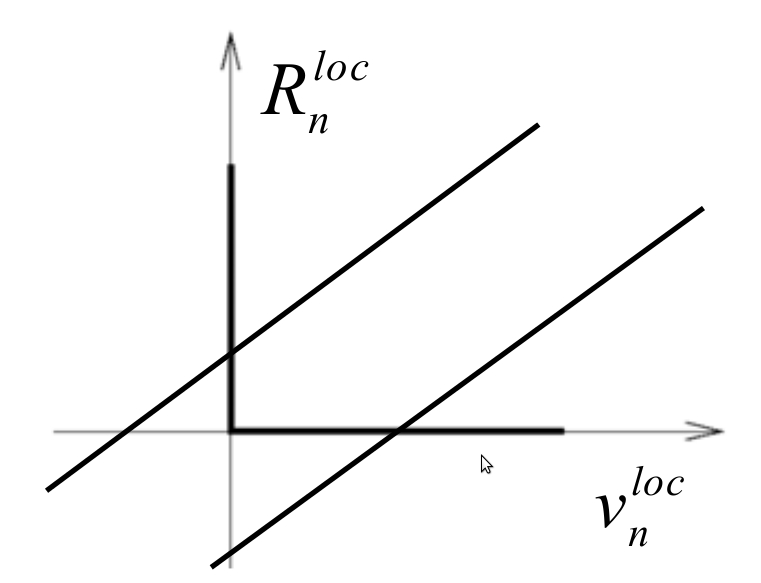
\includegraphics[width=.85\textwidth]{pics/contact_dynamics1.jpeg}
  \captionof{figure}{Graphical interpretation}
  \label{fig:signorini3}
\end{minipage}
\end{minipage}
\vspace{0.1cm}

We can divide the possible cases into
\begin{itemize}
\item Particles are not in contact,
\item Particles are in closing contact,
\item Particles are in persisting contact and
\item Particles are in opening contact.
\end{itemize}


If the particles are not in contact at all, we can ignore the forces. If the particles are getting closer, one has to check if there is an overlap in every time step. If there is no contact then one doesn't need to calculate any force, but if there is a contact one has to apply the constraint forces. If there is an overlap, we have to make sure that the local velocity is such that after the time step the two objects are just in contact and not overlapping. This can be done by changing the slope in \eqref{eq:r_loc} that depends on $\Delta t$. This means that one integrates only until the moment in which the particles touch. After that, the forces are applied in the following time step. In the case of the persisting contact one can calculate the force according to \eqref{eq:r_loc} so that the contact coordinates won't change in the next time step.


In 3D, velocities and forces are given by vectors:

\begin{equation*}
\vec{v}_{1,2}= \cvvec{v^x_{1,2}}{v^y_{1,2}}{v^z_{1,2}}, 
\hspace{.5cm} 
\vec{R}_{1,2} = \cvvec{R^x_{1,2}}{R^y_{1,2}}{R^z_{1,2}}, 
\hspace{.5cm} 
\vec{F}^{\text{ext}}_{1,2} = \cvvec{F^{x,\text{ext}}_{1,2}}{F^{y, \text{ext}}_{1,2}}{F^{z, \text{ext}}_{1,2}}
\end{equation*}

\noindent
In order to formulate the problem in a simpler way, we can project all the variables onto the normal vector:

$$
\vec{n}= \cvvec{n^x}{n^y}{n^z}
\hspace{.5cm} 
{v}^{loc}_n = \vec{n} \cdot \kl{\vec{v}_2 - \vec{v}_1}, 
\hspace{.5cm}
\vec{R}_1= -\vec{n} R^{loc}_n,
\hspace{.5cm}
\vec{R}_2= \vec{n} R^{loc}_n
$$

From the projection we can obtain the matrix $H$ for the coordinate transformation,
$$
v_n^{loc} = H^T\cvec{\vec{v}_1}{\vec{v}_2},
\hspace{.5cm}
\cvec{\vec{v}_1}{\vec{v}_2} = HR^{loc}_n
$$


$$
\Rightarrow \hspace{.4cm} H^T = \kl{-n_x, -n_y, -n_z,n_x,n_y,n_z }
$$



This technique implies dissipation. Energy is not conserved, since forces are created artificially. Collisions are completely plastic, and after a contact particles stick together.




\subsection{Many-body Contact Dynamics}




We will formulate now the problem for $N$ contact particles. For this the coordinates have to be generalized to a set of variable for the entire system:


\begin{align*}
\dot{q} &= \kl{\vec{v}_1,\vec{\omega}_1,...,\vec{v}_N,\vec{\omega}_N}\\
R       &= \kl{\vec{R}_1,\vec{T}_1,...,\vec{R}_N,\vec{T}_N}\\
F^{\,\text{ext}} &= \kl{\vec{F}^{\,\text{ext}}_1,0,...,\vec{v}^{\,\text{ext}}_N,0}\\
\end{align*}


The number of components depends on the dimension of the simulated system. In 2D, there are for each particle 2 transational and one rotational degrees of freedom, hence 3$N$ total components. In 3D every particle has 3 translational and 3 rotational degrees of freedom. In any case, the number of contacts does not necessarily equal the number of particles. Let $c$ be the number of contacts (mind that every particle can be in contact with more than one particle!). In 2D we will have $2c$ components of contact variables (1 normal and 1 tangential), while in  3D we have $3c$ components (1 normal and 2 tangential). Neglecting torques at the contact points leads to:

$$
\vec{u}= \cvvec{\vec{v}^{\,\text{loc}}_1}{\text{...}}{\vec{v}^{\,\text{loc}}_c}
\hspace{.5cm} 
\vec{R}^{\,\text{loc}}= \cvvec{\vec{R}^{\,\text{loc}}_1}{...}{\vec{R}^{\,\text{loc}}_c}
$$



At every time step, the kind of contact between the particles and the particles in contact change. The matrix that transforms our standard variables into contact variables ($H$) is therefore not constant.  Mind that H is given by a $2c\times3N$ matrix in 2D and $3c\times6N$ in 3D. Taking for the sake of simplicity the 2D case, we can write the problem as

\begin{equation*}
u= H^T \dot{q}, 
\hspace{0.5cm}
R= HR^{\,\text{loc}}
\end{equation*}
As already mentioned, the matrix $H$ has to be updated at every time step. Defining the diagonal mass matrix $M$ as

\begin{equation*}
M \equiv
 \begin{pmatrix}
  \xi_1 	&  \cdots & 0 \\
  \vdots&  \ddots & \vdots  \\
  0 	&  \cdots & \xi_N
 \end{pmatrix}
\end{equation*}
with

\begin{equation*}
\xi_i \equiv
 \begin{pmatrix}
  m_i 	&  0 	& 0 \\
  0 	&  m_i	& 0  \\
  0 	&  0 	& I_i
 \end{pmatrix}
\end{equation*}
simplifies the form of the equation of motion:


\begin{equation*}
M\ddot{q}\kl{t} = R\kl{t} + F^{\,\text{ext}}.
\end{equation*}
For each contact, the relation between the contact quantities is then



\begin{equation}
\dot{u}= H^T M^{-1} H R^{\,\text{loc}} + H^TM^{-1}F^{\,\text{ext}}
\label{eq:cont_equation} 
\end{equation}



We can further simplify the equation defining an \emph{effective inverse mass matrix}:

\begin{equation*}
M^{-1}_{\text{eff}}  \equiv  H^TM^{-1}F^{\,\text{ext}}.
\end{equation*}
With this definition we can build an algorithm to solve the equation of motion in the reference frame of the contact variables. Using the implicit Euler integration\footnote{see \citet{comp_phys}} we can rewrite \eqref{eq:cont_equation}:



\begin{equation}
R^{\,\text{loc}} \kl{t+ \Delta t} =  M_{\text{eff}}  \frac{u\kl{t+\Delta t}-u^{\,\text{free}}\kl{t+\Delta t}}{\Delta t}
\end{equation}

Mind that the dimension of the system we are solving (the particles in contact) changes over time. This is a very unusual situation and it carries difficulties. Another main problem in the method is that the system  of equations that we are solving does not have a unique solution. For an intuition one can think of a chair with four or more legs. The distribution of the weight is not unique. Although we know that if the chair is not strongly asymmetric, then the weight will be distributed equally but mathematically this is not the sole solution. To avoid this problem usually the solution is found iteratively by regarding neighboring contacts as external forces.


Friction, rolling friction, cohesion can be simulated by changing the graphs we discussed at the beginning of the section (See Fig. \ref{fig:signorini} and \ref{fig:signorini2}). As an example, an attractive force within a finite range that can be broken by external forces can be simulated in such a model. This is also important to foresee the plastic properties of objects and materials. The shape of particles and objects plays an important role in industrial design. All the devices that we have today  (cars, bridges, airplanes, etc...) and their components are designed and studied with computer-aided techniques before reaching the production, and then  many iterations alternated with corrections and further simulations are done before any product can land on the market. From the simplest plastic toys to the most complicated objects, all the products are (or at least should be) tested for their properties. In case of interest, in \citet{comp_phys} 3D modelling techniques (such as CAD) are treated more in detail.























